\documentclass[11pt,a4paper]{article}

\usepackage[utf8]{inputenc}
\usepackage[T1]{fontenc}
\usepackage{lmodern}
\usepackage[margin=2.5cm]{geometry}
\usepackage{amsmath,amssymb,amsthm}
\usepackage{graphicx}
\usepackage{booktabs}
\usepackage{hyperref}
\usepackage{natbib}
\usepackage{microtype}
\usepackage{caption}
\usepackage{subcaption}
\usepackage{xcolor}
\usepackage{enumitem}

\hypersetup{
  colorlinks=true,
  linkcolor=blue!60!black,
  citecolor=blue!60!black,
  urlcolor=blue!60!black
}

\title{\textbf{Under What Conditions Does Cooperation Emerge Among Self-Interested Agents?}\\[0.4em]
\large An Illustrative Agent-Based Study with the Prisoner's Dilemma}
\author{Scott Brodie Forsyth}
\date{\today}

\newtheorem{proposition}{Proposition}

\begin{document}
\maketitle

\begin{abstract}
Self-interested agents---individuals who rationally pursue their own payoffs---face a puzzle: in many one-shot social dilemmas, mutual defection is the unique Nash equilibrium, yet cooperation is widespread in nature and human societies. This paper synthesizes canonical game-theoretic and evolutionary mechanisms and supplements them with reproducible Python simulations. The analysis shows, both analytically and computationally, that cooperation can \emph{emerge and persist} only when the strategic environment satisfies additional structure: repeated interaction with a sufficiently high discount factor, spatial or network localization, positive assortment (including kinship), or institutions that alter incentives. The simulations are \textbf{illustrative}: they demonstrate comparative statics consistent with established theory but do \textbf{not} identify causal effects in observational data, nor do they substitute for laboratory or field experiments. The contribution is pedagogical and methodological---a transparent bridge between formal models and visual intuition for readers without specialist training.
\end{abstract}

\section{Introduction}

Imagine two farmers sharing an irrigation canal. Each can contribute labor to maintain it or free-ride on the other's effort. If they interact once and never meet again, standard game theory predicts both will shirk: defection is a dominant strategy in the one-shot Prisoner's Dilemma (PD). Yet real communities often cooperate---sometimes reliably, sometimes fragilely. The central question is therefore not \emph{whether} self-interest exists, but \textbf{under what conditions self-interest leads to cooperation rather than mutual harm}.

This study addresses that question at two levels. First, it states precise mathematical conditions from repeated-game theory and evolutionary biology. Second, it implements agent-based models in Python to visualize how cooperation rises or collapses when those conditions change. Throughout, three types of claims are kept distinct:
\begin{enumerate}[noitemsep]
  \item \textbf{Theoretical claims} (e.g., folk-theorem logic): valid given stated assumptions.
  \item \textbf{Simulation patterns}: numerical illustrations of theory, not independent empirical proof.
  \item \textbf{Empirical generalizations} about humans: supported by literatures cited here but not replicated in this study.
\end{enumerate}

\section{The One-Shot Prisoner's Dilemma}

\subsection{Payoffs and the social dilemma}

Two players simultaneously choose Cooperate ($C$) or Defect ($D$). Payoffs satisfy $T > R > P > S$ and $2R > T + S$, where $T$ is temptation, $R$ reward, $P$ punishment, and $S$ sucker's payoff. The baseline calibration is $T=5$, $R=3$, $P=1$, $S=0$ (Figure~\ref{fig:payoff}).

\begin{figure}[htbp]
  \centering
  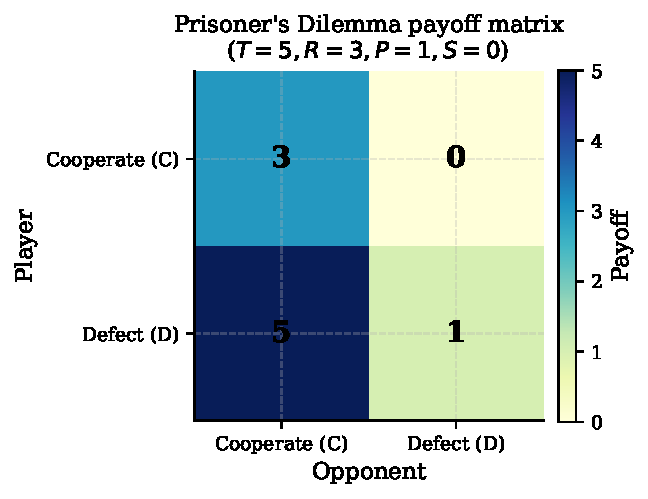
\includegraphics[width=0.42\textwidth]{figures/fig01_payoff_matrix.pdf}
  \caption{Stage-game payoff matrix. Mutual cooperation yields $(3,3)$; unilateral defection yields $(5,0)$ or $(0,5)$; mutual defection yields $(1,1)$.}
  \label{fig:payoff}
\end{figure}

The payoff matrix is
\begin{equation}
  \Pi = \begin{pmatrix} R & S \\ T & P \end{pmatrix},
  \label{eq:matrix}
\end{equation}
where rows index the focal player's action and columns the opponent's.

\subsection{Nash equilibrium in one shot}

Defection strictly dominates cooperation: regardless of the opponent's action, $D$ yields higher payoff ($T > R$ and $P > S$). Hence the unique pure-strategy Nash equilibrium is $(D,D)$ with payoffs $(P,P)$, which is Pareto-dominated by $(C,C)$. This is the canonical \emph{social dilemma}: individual rationality conflicts with collective welfare \citep{hardin1968,binmore1994}.

\paragraph{Plain-language summary.} If people meet once, never interact again, and care only about immediate payoff, cooperation should unravel. Real life often violates at least one of these premises---and that is where cooperation becomes possible.

\section{Mechanisms That Enable Cooperation}

Following \citet{nowak2006} and \citet{west2007}, five mechanism families organize the discussion. Table~\ref{tab:mechanisms} maps each to a qualifying condition.

\begin{table}[htbp]
  \centering
  \caption{Five routes to cooperation among self-interested agents \citep{nowak2006}}
  \label{tab:mechanisms}
  \begin{tabular}{@{}lll@{}}
    \toprule
    Mechanism & Qualifying condition & Intuition \\
    \midrule
    Kin selection & Relatedness $r$ high; $rb > c$ & Help copies of own genes \\
    Direct reciprocity & Repeated play; high $\delta$ & Today's help buys tomorrow's help \\
    Indirect reciprocity & Reputation observability & Cooperators gain social standing \\
    Network reciprocity & Local interaction & Cooperators cluster and protect each other \\
    Group selection & Between-group variance & Groups of cooperators outcompete defectors \\
    \bottomrule
  \end{tabular}
\end{table}

\subsection{Direct reciprocity and repeated games}

When the PD is repeated with discount factor $\delta \in (0,1)$, players can condition future play on past actions. Consider \emph{grim trigger}: cooperate until the opponent defects, then defect forever. Mutual cooperation is a subgame-perfect equilibrium if the stream from cooperation exceeds the one-shot gain from defection:
\begin{equation}
  \frac{R}{1-\delta} \;\ge\; T + \frac{\delta P}{1-\delta}.
  \label{eq:grim}
\end{equation}
Rearranging yields the sharp threshold
\begin{equation}
  \delta \;\ge\; \delta^* \equiv \frac{T-R}{T-P}.
  \label{eq:delta-star}
\end{equation}

\begin{proposition}[Grim-trigger cooperation threshold]
Under perfect monitoring and the payoffs in \eqref{eq:matrix}, mutual cooperation sustained by grim trigger is a subgame-perfect equilibrium of the infinitely repeated PD if and only if $\delta \ge (T-R)/(T-P)$.
\end{proposition}

\begin{proof}[Proof sketch]
If both players cooperate, each receives $R/(1-\delta)$. A unilateral deviation yields $T$ in the current period and $P$ in every subsequent period, totaling $T + \delta P/(1-\delta)$. Cooperation is optimal when $R/(1-\delta) \ge T + \delta P/(1-\delta)$, which rearranges to \eqref{eq:delta-star}. The converse holds by the same comparison. See \citet{fudenberg1991} for the general folk-theorem framework.
\end{proof}

For the baseline payoffs, $\delta^* = (5-3)/(5-1) = 0.5$. Figure~\ref{fig:grim} plots this feasibility region.

\begin{figure}[htbp]
  \centering
  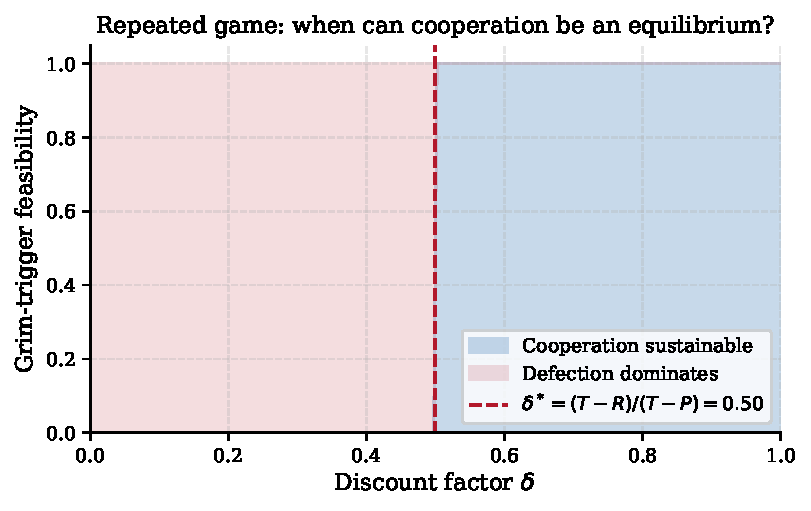
\includegraphics[width=0.62\textwidth]{figures/fig02_grim_trigger.pdf}
  \caption{Grim-trigger cooperation is sustainable for $\delta \ge \delta^*$. Below the threshold, defecting once and returning to mutual punishment is preferable to continued cooperation.}
  \label{fig:grim}
\end{figure}

\citet{axelrod1981} showed in computer tournaments that \emph{Tit-for-Tat}---cooperate first, then mirror the opponent---performs well in repeated PDs with uncertain horizon. However, \citet{press2012} later showed that extortionate strategies can dominate in evolutionary settings, indicating that ``nice'' reciprocity is not the only equilibrium outcome. This study does not resolve equilibrium selection; it characterizes only \emph{when cooperation is \textbf{possible}}.

\subsection{Kin selection and positive assortment}

Hamilton's rule states that a costly cooperative act can spread by natural selection when
\begin{equation}
  rb > c,
  \label{eq:hamilton}
\end{equation}
where $r$ is genetic relatedness between actor and recipient, $b$ is benefit to recipient, and $c$ is cost to actor \citep{hamilton1964,trivers1971}. Mapping the PD to a donation game with benefit $b = R - P$ and cost $c = T - R$ yields the threshold $r > c/b = (T-R)/(R-P)$. Under the baseline payoffs, $r^* = 2/2 = 1$: kin selection alone requires maximal relatedness unless payoffs are rescaled. \emph{Positive assortment}---non-random pairing of cooperators---plays an analogous role in behavioral and cultural evolution \citep{lehmann2006}.

Figure~\ref{fig:relatedness} reports a stylized group model in which cooperation rises with an assortment parameter $r$. The dashed vertical line marks the Hamilton threshold under the donation framing; the simulation parameter is a behavioral assortment rate, not a direct estimate of genetic relatedness, so the line is a theoretical benchmark rather than a predicted breakpoint.

\begin{figure}[htbp]
  \centering
  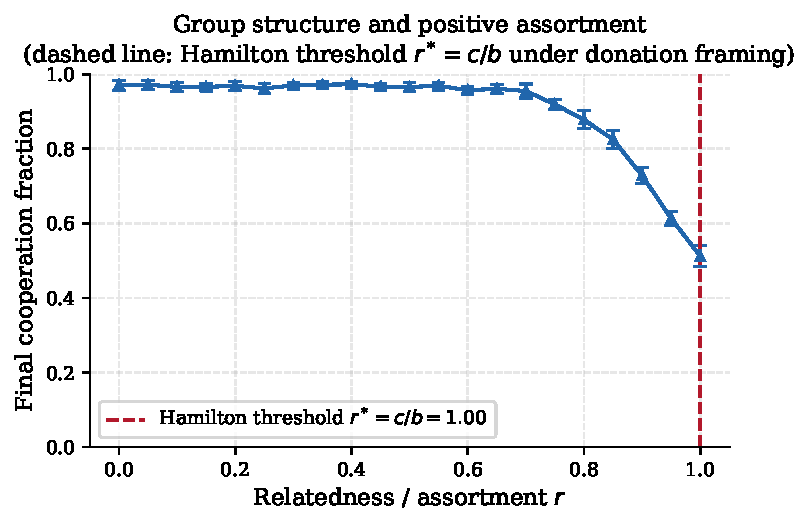
\includegraphics[width=0.62\textwidth]{figures/fig08_relatedness_sweep.pdf}
  \caption{Cooperation fraction vs.\ assortment in a group-structured simulation (10 replicates per point). The dashed line marks the Hamilton threshold $r^*=c/b=1$ under the baseline payoff calibration (donation framing).}
  \label{fig:relatedness}
\end{figure}

\subsection{Spatial and network reciprocity}

When interactions are \emph{local}---on a lattice or network---cooperators can form clusters that earn high payoffs from each other while isolating exploiters \citep{nowak1992,szabo2007}. \citet{nowak1992} showed that spatial structure can sustain cooperation even when well-mixed populations cannot.

Figures~\ref{fig:spatial}--\ref{fig:mixed} contrast spatial and well-mixed dynamics.

\begin{figure}[htbp]
  \centering
  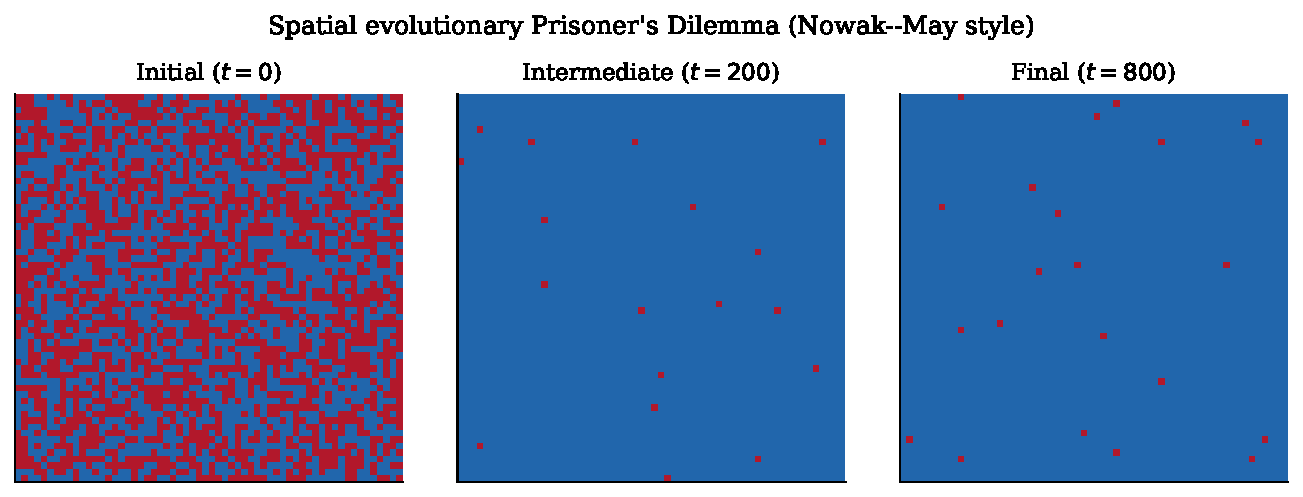
\includegraphics[width=0.95\textwidth]{figures/fig03_spatial_snapshots.pdf}
  \caption{Snapshots of a spatial evolutionary PD on a $60 \times 60$ toroidal lattice. Cooperators (blue) and defectors (red) self-organize into clusters; boundaries are dynamic.}
  \label{fig:spatial}
\end{figure}

\begin{figure}[htbp]
  \centering
  \begin{subfigure}[b]{0.48\textwidth}
    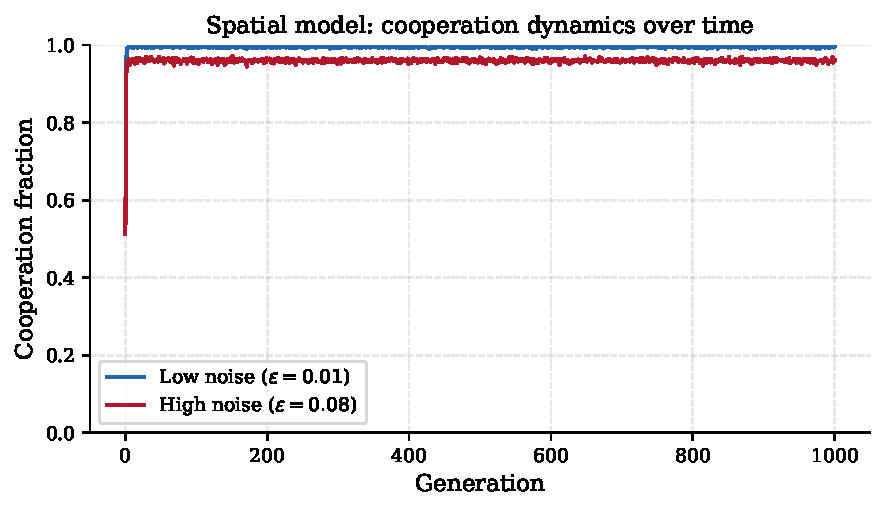
\includegraphics[width=\textwidth]{figures/fig04_spatial_timeseries.pdf}
    \caption{Effect of noise}
  \end{subfigure}
  \hfill
  \begin{subfigure}[b]{0.48\textwidth}
    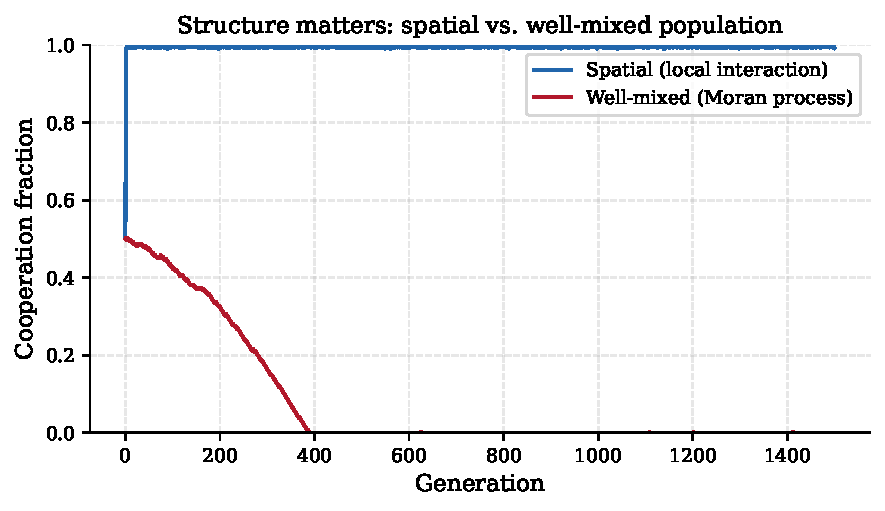
\includegraphics[width=\textwidth]{figures/fig07_mixed_vs_spatial.pdf}
    \caption{Spatial vs.\ well-mixed}
  \end{subfigure}
  \caption{Left: higher strategy noise ($\varepsilon$) erodes cooperation. Right: identical payoffs but different population structure yield opposite long-run outcomes in a representative run (seed fixed).}
  \label{fig:mixed}
\end{figure}

\subsection{Institutions and punishment}

Self-interest can also support cooperation when rules change payoffs. \citet{ostrom1990} documented how communities govern commons through monitoring, graduated sanctions, and conflict-resolution mechanisms---not through naive altruism. Laboratory evidence shows that \emph{altruistic punishment} of defectors can sustain cooperation in public-goods games \citep{fehr2002}, though punishment itself is costly and culturally variable \citep{henrich2001}. Institutional design is not simulated here; it is noted as a distinct, empirically important channel.

\section{Computational Methods}

All code is in \texttt{src/simulation.py} and \texttt{src/generate\_figures.py}. Models include:
\begin{itemize}[noitemsep]
  \item \textbf{Spatial PD}: $50 \times 50$ toroidal lattice, von Neumann neighbors, synchronous imitate-best-neighbor update with noise $\varepsilon \in [0,1]$.
  \item \textbf{Well-mixed Moran process}: fitness-proportional imitation with mutation rate $0.01$.
  \item \textbf{Group assortment}: reproduction with probability $r$ of copying a randomly chosen within-group member.
  \item \textbf{Parameter sweeps}: temptation $T$, noise $\varepsilon$, assortment $r$; 10--12 independent replicates per grid point; error bars are approximate 95\% confidence intervals ($\pm 1.96 \times \text{SE}$).
\end{itemize}

Random seeds are fixed for reproducibility. Simulations run for 250--1500 generations depending on the model. Outputs are \textbf{not} calibrated to field data; they illustrate theoretical comparative statics.

\section{Results: Comparative Statics}

Figure~\ref{fig:temptation} varies temptation $T$ while holding $R=3$, $P=1$, $S=0$. As defection becomes more lucrative, cooperation eventually collapses---consistent with the comparative static that higher $T$ shrinks the basin of attraction for cooperative clusters \citep{nowak1992}.

\begin{figure}[htbp]
  \centering
  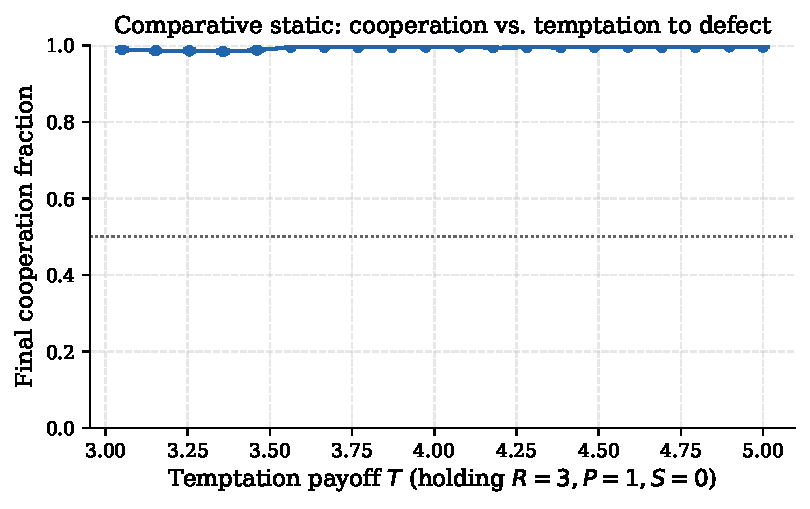
\includegraphics[width=0.62\textwidth]{figures/fig05_temptation_sweep.pdf}
  \caption{Final cooperation vs.\ temptation $T$ in the spatial model (12 replicates per point).}
  \label{fig:temptation}
\end{figure}

Figure~\ref{fig:noise} shows that execution errors and mutation ($\varepsilon$) reduce cooperation on average, consistent with the idea that reciprocity requires sufficiently accurate memory and implementation \citep{nowak2010structured}. The relationship need not be strictly monotonic at every point because of stochastic cluster dynamics.

\begin{figure}[htbp]
  \centering
  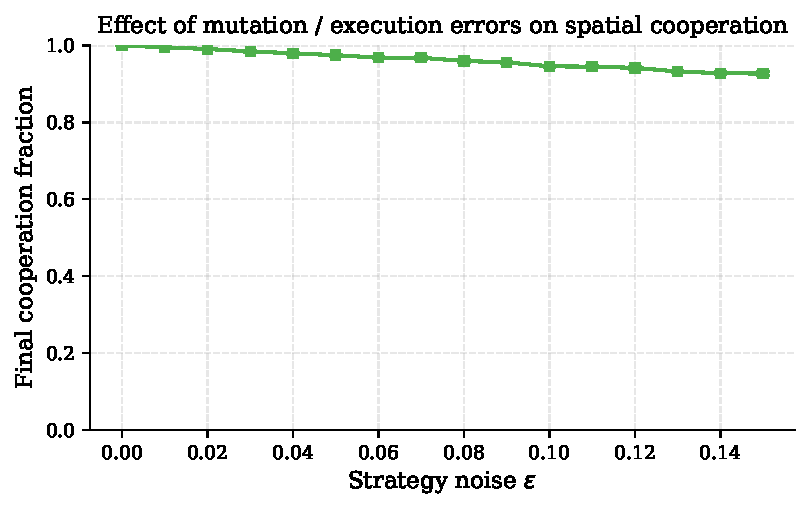
\includegraphics[width=0.62\textwidth]{figures/fig06_noise_sweep.pdf}
  \caption{Noise erodes cooperative clusters by introducing defector invasions (10 replicates per point).}
  \label{fig:noise}
\end{figure}

Figure~\ref{fig:summary} aggregates illustrative outcomes across mechanisms. One-shot play and well-mixed evolution yield low cooperation; repeated-game feasibility (here $\delta=0.8 > \delta^*$), spatial structure, and positive assortment yield high cooperation \emph{under the parameterizations used here}.

\begin{figure}[htbp]
  \centering
  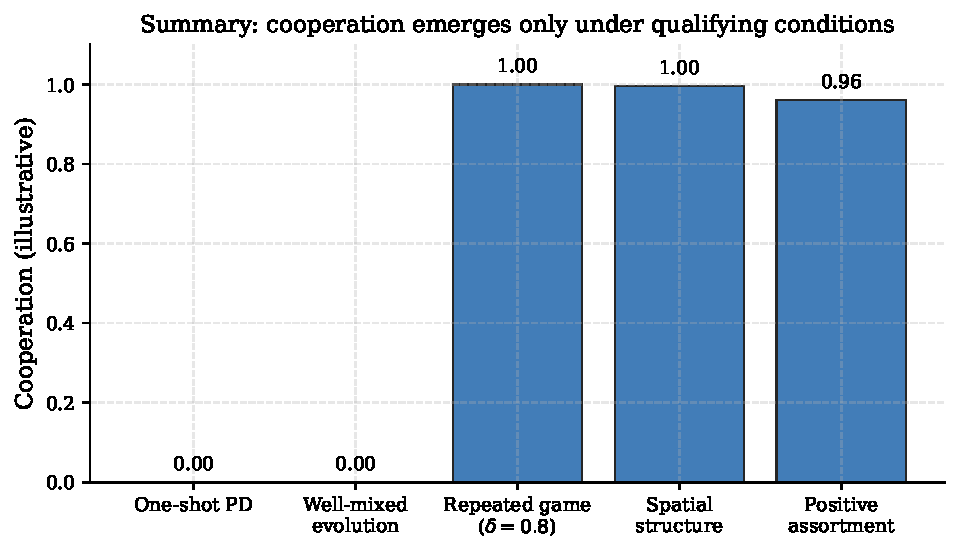
\includegraphics[width=0.72\textwidth]{figures/fig09_mechanisms_summary.pdf}
  \caption{Illustrative cooperation levels by mechanism. Spatial, well-mixed, and assortment bars come from single-seed simulation runs; the one-shot bar is the Nash prediction (0); the repeated-game bar marks grim-trigger feasibility at $\delta=0.8$.}
  \label{fig:summary}
\end{figure}

\section{Scope, Claims, and Limitations}

\subsection{What this study establishes}

\begin{enumerate}[noitemsep]
  \item \textbf{Logical necessity in models}: In the one-shot PD, defection is dominant; cooperation requires modifying the game (repetition, assortment, structure, or institutions).
  \item \textbf{Quantitative thresholds}: Equations~\eqref{eq:delta-star} and~\eqref{eq:hamilton} give explicit parameter boundaries for two canonical mechanisms.
  \item \textbf{Qualitative simulation patterns}: Spatial localization and low noise tend to promote cooperation; high temptation and well-mixed interaction tend to suppress it---patterns aligned with \citet{nowak1992,nowak2006}.
\end{enumerate}

\subsection{Limitations}

\begin{enumerate}[noitemsep]
  \item \textbf{No empirical identification.} The simulations are \emph{stylized models}, not estimates of causal effects in field data. No claim is made that, for example, ``raising relatedness by 0.1 \emph{causes} a 15\% cooperation increase'' in human populations.
  \item \textbf{Binary strategies.} Real behavior is continuous (partial contributions, negotiation, hybrid norms). Binary $C/D$ is a deliberate simplification.
  \item \textbf{Equilibrium selection.} Many strategy profiles can coexist in repeated and spatial games; the imitative dynamics implemented here select particular trajectories without general uniqueness \citep{fudenberg1991,press2012}.
  \item \textbf{Parameter dependence.} Spatial cooperation persists for some $(T,R,P,S)$ combinations and vanishes for others \citep{nowak1992}. The sweeps cover a subset of parameter space only.
  \item \textbf{Human motives.} Experiments document fairness, guilt, and parochialism beyond material PD payoffs \citep{henrich2001,rand2013}. Homo economicus is a modeling device, not a complete psychological account.
  \item \textbf{External validity.} Results from $50 \times 50$ lattices may not transfer to large heterogeneous networks, mobile populations, or institutional settings with courts and contracts.
\end{enumerate}

\section{Conclusion}

This study maps the conditions under which cooperation can emerge from self-interest: repeated interaction (with $\delta \ge (T-R)/(T-P)$), positive assortment (Hamilton's $rb > c$), spatial or network structure, and institutional enforcement. Python agent-based models illustrate these comparative statics with transparent, reproducible code. The analysis is intentionally bounded: it clarifies \emph{when} and \emph{why} cooperation is theoretically sustainable, while leaving empirical measurement of those conditions in specific societies to field work and experiments \citep{ostrom1990,fehr2002,henrich2001}.

\section*{Replication}

\begin{verbatim}
pip install -r requirements.txt
python src/validate.py
python src/generate_figures.py
cd paper && pdflatex cooperation_emergence && bibtex cooperation_emergence
pdflatex cooperation_emergence && pdflatex cooperation_emergence
\end{verbatim}

\bibliographystyle{apalike}
\bibliography{references}

\end{document}
